\setchapterpreamble[u]{\margintoc}
\chapter{Equazione di Schrödinger}
\labch{schroedinger}

\section{Esercizi}

\subsection{Esercizio 16}

\paragraph{Nozioni teoriche}

%TODO: scrivere nozioni teoriche

Si ottiene dunque, nel caso particolare del problema:

\[
	\left[-\frac{N^2}{16}K+\mathcal{V}\right]\phi = \mathcal{E} \phi \quad \mathcal{E} = EL, \mathcal{V} = VL
\]

con $K_{ii} = -2, K_{j+1,j}=K_{j,j+1}=1 \quad 0 \leq j < N-1, \; 0 \leq i < N$. \\$V= -V_0$ per $1/4 \leq x \leq 3/4$


\paragraph{Implementazione}

\label{file}
\subparagraph{File necessari} \texttt{ex\_16.cpp}

L'implementazione segue direttamente dalla equazione sopracitata applicando il \textit{Power Deflation Method}

\paragraph{Analisi dei risultati e conclusioni}

\begin{enumerate}

	\item Si veda \texttt{ex\_16.cpp}

	\item

	      \begin{marginfigure}
		      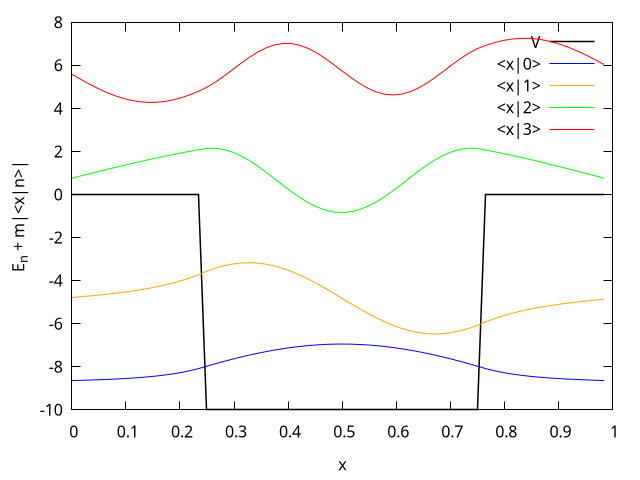
\includegraphics[width=1.5\textwidth]{schroedinger_1_1.png}
		      \caption{Autofunzioni della buca finita di potenziale}
		      \label{fig:schroedinger_1_1}
	      \end{marginfigure}

	      Come ci si aspetta si ottengono stati legati che qualitativamente possono essere considerati corretti: i nodi corrispondono all'energia dello stato; all'interno della parete la funzione d'onda scala come un'esponenziale; nei casi al di sopra della parete si ottengono oscillazioni a frequenza piu' alta per $E-V$ piu' grandi.


	\item
	      \begin{marginfigure}
		      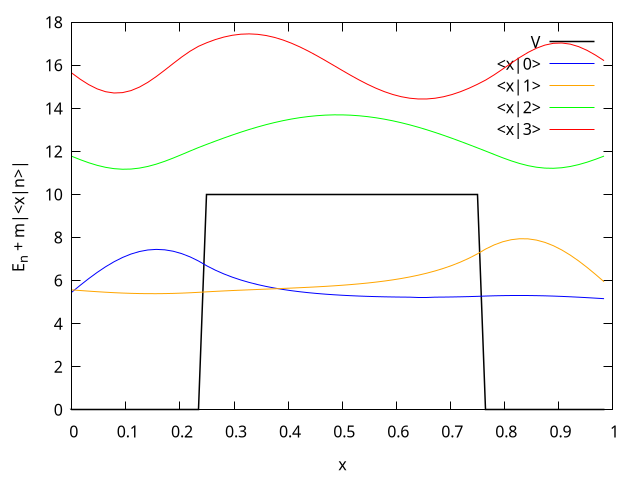
\includegraphics[width=1.5\textwidth]{schroedinger_1_2.png}
		      \caption{Autofunzioni della buca finita di potenziale}
		      \label{fig:schroedinger_1_2}
	      \end{marginfigure}
	\item


	      \begin{marginfigure}
		      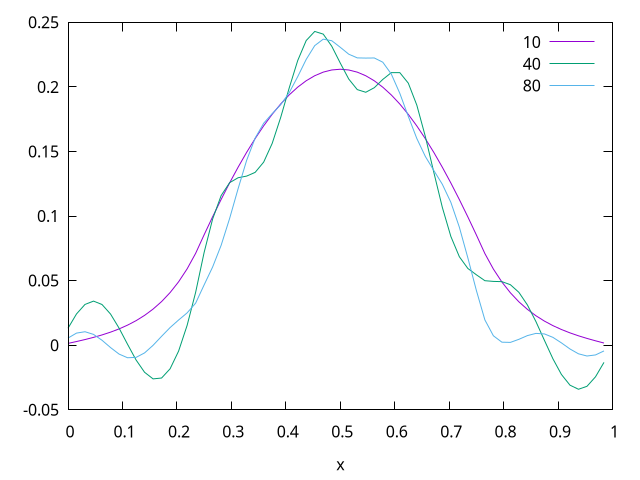
\includegraphics[width=1.5\textwidth]{schroedinger_1_3.png}
		      \caption{Autofunzioni della buca finita di potenziale}
		      \label{fig:schroedinger_1_3}
	      \end{marginfigure}
	\item


	      \begin{marginfigure}
		      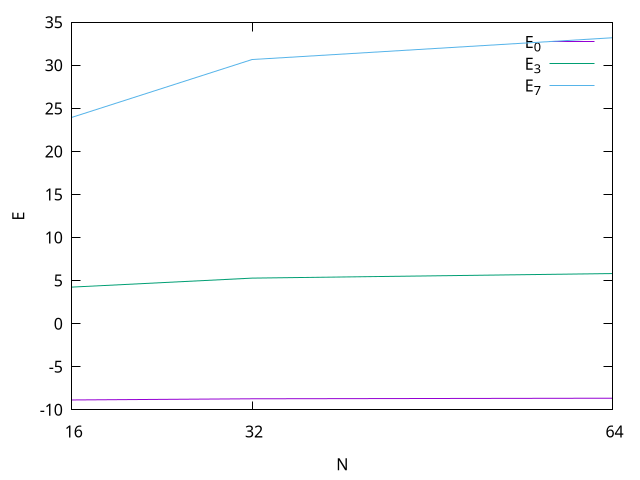
\includegraphics[width=1.5\textwidth]{schroedinger_1_4.png}
		      \caption{Autofunzioni della buca finita di potenziale}
		      \label{fig:schroedinger_1_4}
	      \end{marginfigure}

\end{enumerate}

\subsection{Esercizio 17}

\paragraph{Nozioni teoriche}

\paragraph{Implementazione}

\paragraph{Analisi dei risultati e conclusioni}






